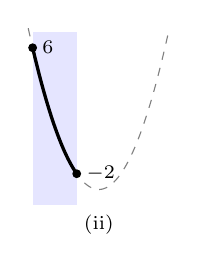
\begin{tikzpicture}[x=2.8mm,y=2mm]
\fill[blue!10] (-1,-4) rectangle (1,7);
\ax{-1.6}{5.6}{-4}{7}
\draw[dashed,gray,domain=-1.2:5.2,samples=80] plot (\x,{(\x-2)^2-3});
\draw[very thick,domain=-1:1,samples=80] plot (\x,{(\x-2)^2-3});
\fill (-1,6) circle (1.6pt);
\node[right] at (-1,6){\scriptsize 6};
\fill (1,-2) circle (1.6pt);
\node[right] at (1,-2){\scriptsize $-2$};
\node[below] at (current bounding box.south){\scriptsize (ii)};
\end{tikzpicture}